
%%%%%%%%%%%%%%%%%%%%%%%%%%%%%%%%%%%%%%%%%%%%%%%%%%%%%%%%%%%%%%%%%%%%%%%%%%%%%%%
%
%  EGSnrc manual: pegs4 manual
%  Copyright (C) 2015 National Research Council Canada
%
%  This file is part of EGSnrc.
%
%  EGSnrc is free software: you can redistribute it and/or modify it under
%  the terms of the GNU Affero General Public License as published by the
%  Free Software Foundation, either version 3 of the License, or (at your
%  option) any later version.
%
%  EGSnrc is distributed in the hope that it will be useful, but WITHOUT ANY
%  WARRANTY; without even the implied warranty of MERCHANTABILITY or FITNESS
%  FOR A PARTICULAR PURPOSE.  See the GNU Affero General Public License for
%  more details.
%
%  You should have received a copy of the GNU Affero General Public License
%  along with EGSnrc. If not, see <http://www.gnu.org/licenses/>.
%
%%%%%%%%%%%%%%%%%%%%%%%%%%%%%%%%%%%%%%%%%%%%%%%%%%%%%%%%%%%%%%%%%%%%%%%%%%%%%%%
%
%  Author:          Iwan Kawrakow, 2003
%
%  Contributors:    Blake Walters
%                   Ernesto Mainegra-Hing
%                   Frederic Tessier
%
%%%%%%%%%%%%%%%%%%%%%%%%%%%%%%%%%%%%%%%%%%%%%%%%%%%%%%%%%%%%%%%%%%%%%%%%%%%%%%%


%This started as SLAC265.AP3 and is for use in egsnrc_um.tex
%
% Do not try to add section commands since this uses many internal
%cross-references.

% Replace commented line for the one with fixed date when commiting
% Beware: Using the macro below conflicts between CVS and latex!!!
% \lfoot[{\sffamily {\leftmark}}]{{\small Last edited $Date: 2013/01/04 14:38:47 $
\lfoot[{\sffamily {\leftmark}}]{{\small Last edited 2011/05/02 18:36:27
}}


\section{PEGS4 User Manual}
\label{pegs4}


\typeout{PEGS4 User Manual starts here}
The PEGS4 system has been modified very little for use with EGSnrc although
EGSnrc requires considerably more data than provided by PEGS4 and this is
read in directly via the HATCH routine (see fig~\ref{fig_egsnrc_structure}
on page~\pageref{fig_egsnrc_structure}).  Most of this section is basically
a reprint of the PEGS4 User Manual from SLAC-265.  There have been a few
additions to PEGS4 since 1985 and these are summarized in the next section.

In addition to what is described here, the EGSnrcMP environment includes
a user-friendly GUI for using PEGS4. See Report PIRS-877\cite{Ka03}
for a detailed description.
\begin{figure}[ht]
   \begin{center}
%can be left out, but allows figures to be made
   \htmlimage{scale=1.6}{}
   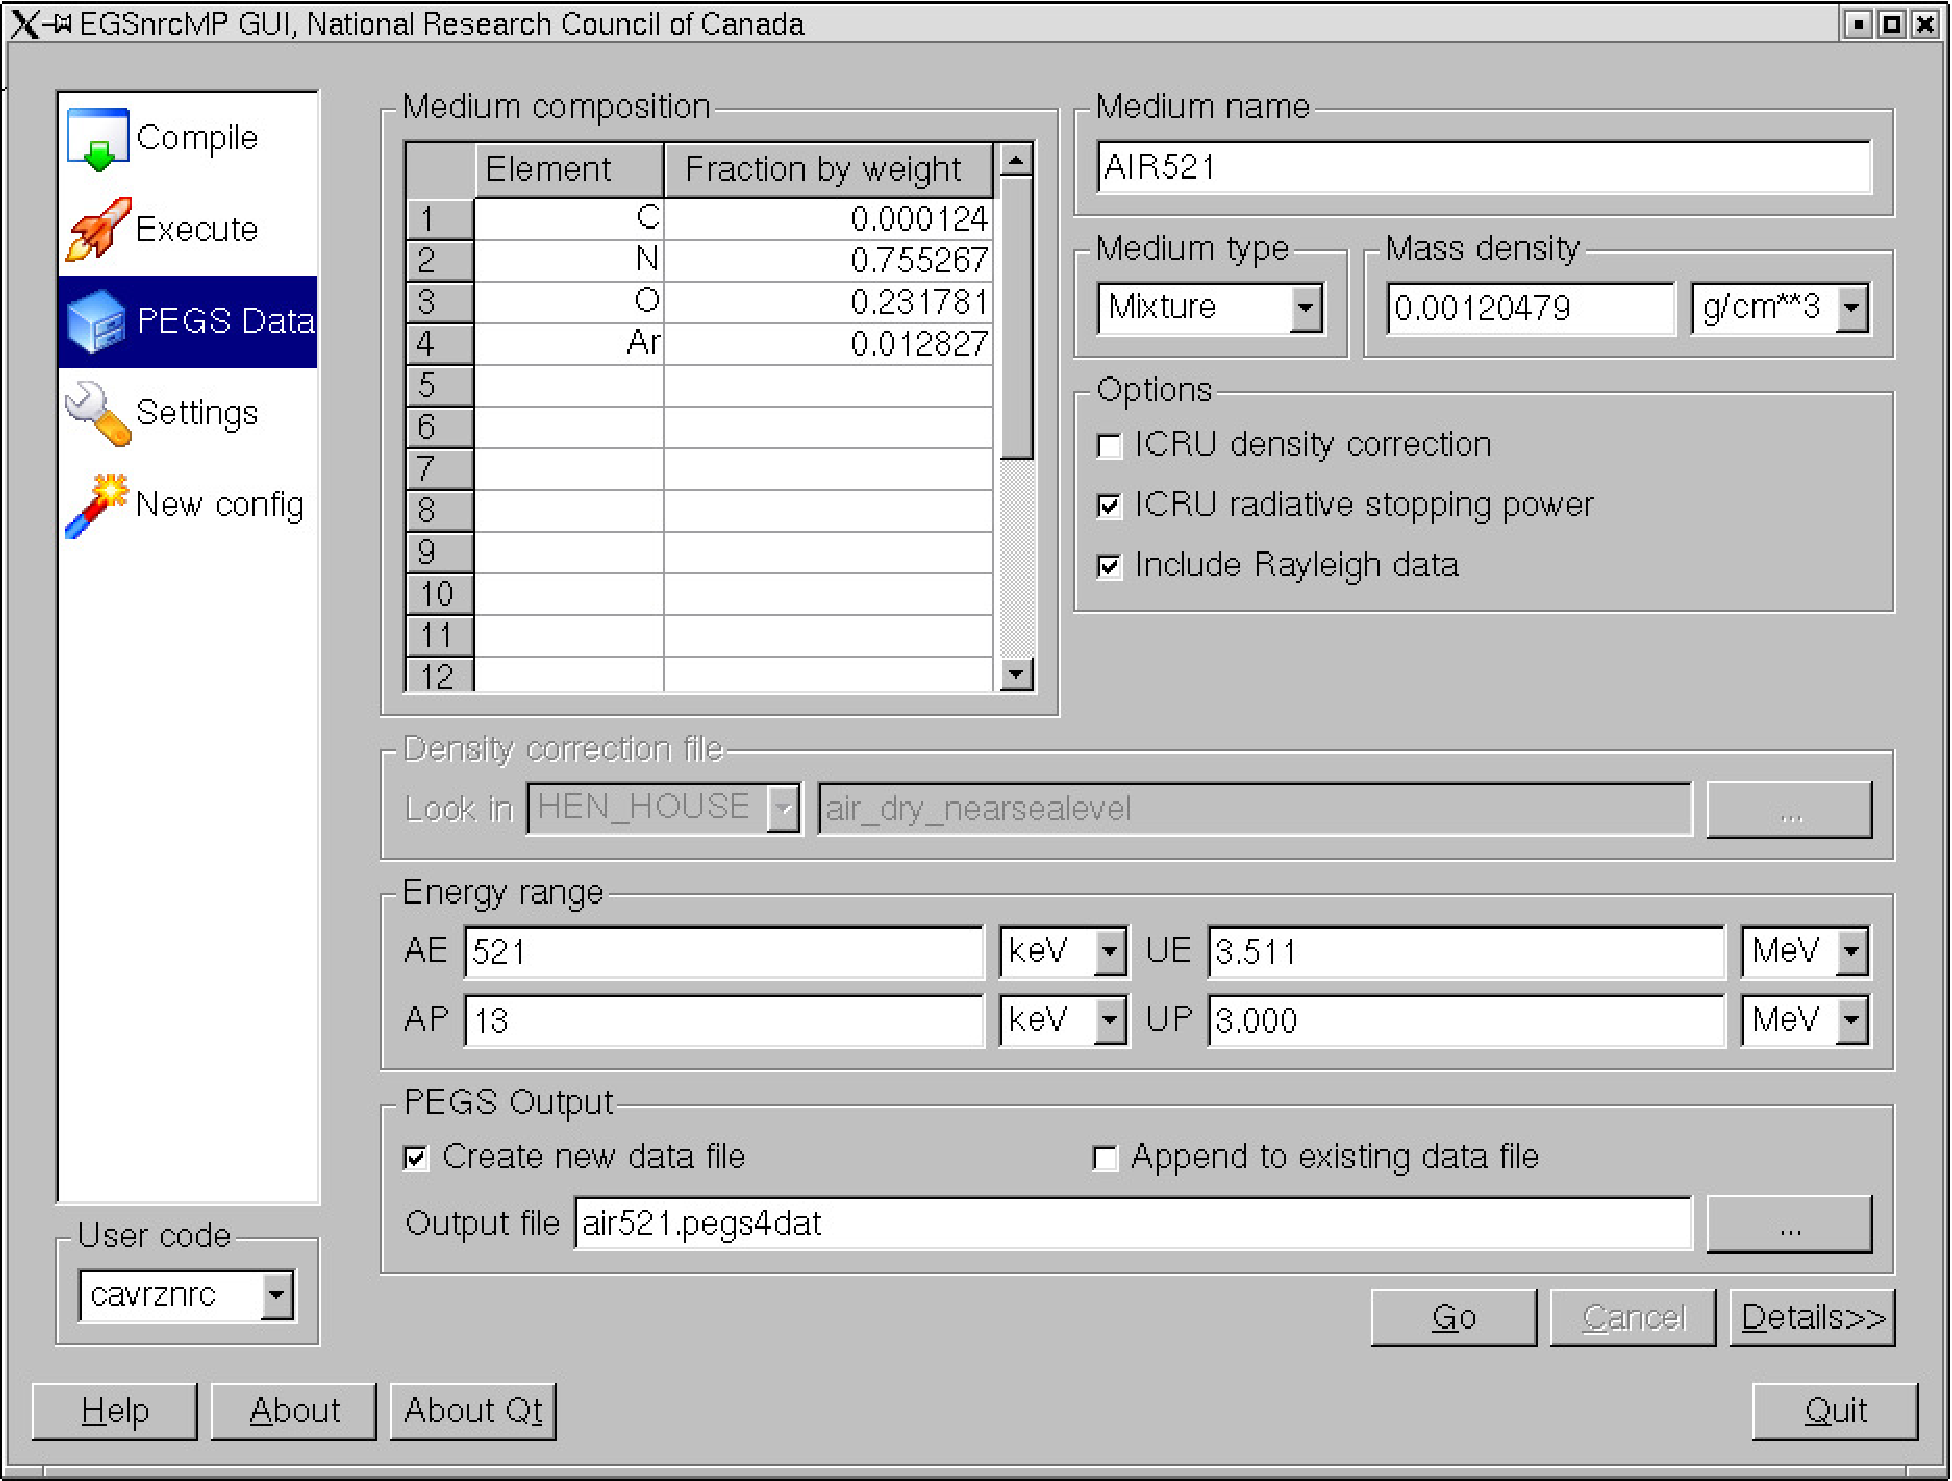
\includegraphics[width=12cm]{figures/egs_gui_pegs4_screen}
    \end{center}
   \caption{Screen shot of the {\tt egs\_gui} set to run PEGS4 to create
an air data set. Filling in this form is much easier than creating an input
file and access to the density effect corrections is easy. The GUI
does not allow any value except {\tt IUNRST = 0}. For details, see
PIRS-877\cite{Ka03}. }
   \label{fig_pegs4_screen}
\end{figure}

\subsection{Some new documentation}

\subsubsection{Photon data for EGSnrc}
\label{xsections}
Originally, EGS main field of application was high energy physics.
For this reason, no attention was paid to the accuracy of the
photon cross sections near atomic absorption edges\cite{RB90} and
PEGS4 was designed to generate a grid with a maximum number of photon
energy points, {\tt \$MXGE}, in the entire energy range requested by the user.
{\tt \$MXGE} is a macro which sets the array dimensions for the energy-dependent
photon data. Although {\tt \$MXGE} can be changed in the PEGS4 code,
PEGS4's algorithm for deciding how many bins to use might still pick many
fewer bins than {\tt \$MXGE}. The decision is based on the overall accuracy to
reproduce the cross sections in the entire energy interval.

\begin{figure}[hbtp]
\begin{center}
\includegraphics*[width=10.0cm]{figures/xcom_250keV_zoom}
\end{center}
\caption[Mean free path $\lambda$ for lead in the vicinity
of the L1 and L2 atomic absorption edges for two different
energy grids]
{Mean free path $\lambda$ for lead in the vicinity
of the L1 and L2 atomic absorption edges for two different
energy grids. Data sets generated by EGSnrc from
the XCOM cross section compilation for an energy range
10 keV to 250 keV.
}
\label{accuracy_xsections}
\end{figure}

Typical PEGS4 data sets used in radiotherapy
calculations are created for an energy range between 10 keV and 20 MeV.
If these data sets are used in the kilovoltage energy
range, inaccuracies in the cross section interpolation procedure near
absorption edges can potentially lead to errors in the calculations.
Fig. \ref{accuracy_xsections} shows two cross section data sets
for the same energy range (10 keV - 250 keV) when using
different energy grids (200 and 2000 bins). A coarser energy
grid will cause larger interpolation errors near the absorption edge.

EGSnrc default behavior has been set to ignore PEGS4 photon
data and recreate the photon cross sections using a logarithmic energy
grid with {\tt \$MXGE} energy points. However, EGSnrc still needs the
PEGS4 data file for material information, photon threshold energies
({\tt AP, UP}), and a fraction of the electron data.
By default data is read from the XCOM\cite{HS95} photon cross section
compilation ({\tt xcom\_pair.data, xcom\_photo.data, xcom\_rayleigh.data and
xcom\_triplet.data}). As alternatives, EGSnrc offers cross section data files
for the Storm and Israel\cite{SI70}({\tt si\_*.data}) and EPDL97\cite{Cu89}
({\tt epdl\_*.data}) photon cross section compilations.
New photon cross section compilations can be added following the
same format as above, \ie, {\tt prefix\_*.data}.
The choice of the photon cross section
compilation is done by input as shown in the example below:
\begin{verbatim}

  :start MC transport parameter:
      .                             # This entry is case sensitive
      Photon cross sections = xcom  # xcom (default), epdl, si or any_prefix
      .
  :stop MC transport parameter:

\end{verbatim}
The prefix used is case sensitive and must be such that the required files
are available in the {\tt \$HEN\_HOUSE/data} directory.

Since the 2011 release (V4-r2-3-2) EGSnrc allows the
use of photon cross section data in the PEGS4 data file. This could
come in handy to compare with older calculations for validation
purposes. To accomplish this, one must set the photon cross section key to
{\tt pegs4} (case insensitive) as shown in the following input file snippet:
\begin{verbatim}

  :start MC transport parameter:
      .
      Photon cross sections = pegs4 # case insensitive
      .
  :stop MC transport parameter:

\end{verbatim}
\subsubsection{Some additional outputs- unrestricted cross sections}
The original version of PEGS4 contained a few undocumented options which
many people have made use of, so they are now documented here.  Basically
there is an additional parameter, {\tt IUNRST} which allows various stopping
powers to be calculated, rather than just the restricted stopping powers
normally calculated when {\tt IUNRST = 0}.  The {\tt IUNRST} input is made as part of
the namelist input for INP (along with NE, AE etc).  Basically {\tt IUNRST} gives
access to a variety of different stopping powers and allows for simulations
which model various types of CSDA calculations.
\begin{description}
\index{IUNRST}
\index{restricted stopping powers}
\index{unrestricted stopping powers}
\index{radiative stopping powers}
\index{collision stopping powers}
\item[IUNRST = 0, restricted stopping powers:] This is the default case
which is needed for normal simulations. The stopping powers output by PEGS4
are the restricted collision and radiative stopping powers.

\item[IUNRST = 1, unrestricted collision stopping power:] This is useful
for calculating unrestricted stopping powers for comparison to frequently
published values.

\item[IUNRST = 2, CSDA data set:] This produces a data set which can do one
form of CSDA calculation. The stopping power produced is the unrestricted
total (collision + radiative) stopping power and the distances to discrete
electron interactions is infinite (i.e. they never occur). A simulation
done with this data set is a form of CSDA calculation, with all of the
bremsstrahlung energy deposited locally.

\item[IUNRST = 3, CSDA calculation with brem interaction:] The stopping
powers are the sum of the unrestricted collision stopping power plus the
restricted stopping power and the distance to discrete interactions takes
into account only bremsstrahlung events.

\item[IUNRST = 4, CSDA calculation with delta-ray interactions:] The
stopping powers are the sum of the restricted collision stopping powers and
the unrestricted collision stopping powers and the distance to discrete
interactions takes into account only the creation of knock-on electrons
or delta-rays.

\item[IUNRST = 5, unrestricted radiative stopping power:] This complements
{\tt IUNRST = 1} and allows comparison to published radiative stopping powers.

\item[IUNRST = 6, restricted radiative stopping power:] Allows for direct
calculation of the restricted radiative stopping powers.

\item[IUNRST = 7, restricted collision stopping powers:] Allows for direct
calculation of the restricted collision stopping power.
\end{description}
Note that for low values of AP (e.g. 0.010 keV) the restricted radiative
collision stopping power is very close to zero and hence the stopping
powers with {\tt IUNRST = 0} are close to those for {\tt IUNRST = 7}.

The code EXAMIN (see section~\ref{examin}, page~\pageref{examin}) will take
the data sets produced by PEGS4 and print tables of cross section data
and/or plot these same data in user friendly units.
\index{EXAMIN}

\subsubsection{Use of ICRU Report 37 Collision Stopping Powers}
\label{icru37_csp}
\index{ICRU Report 37}
\index{collision stopping powers}
For very precise dosimetry work it is often advantageous to make use of
collision stopping powers recommended by the ICRU in their Report
37\cite{ICRU37}.  This option was added to PEGS4 in 1989\cite{Du89}.
Basically PEGS4 allows the user to read in a file which contains an arbitrary
density effect data set ($\delta$ values). The EGSnrc distribution
supplies the data sets
required for a large number of materials as calculated by Berger and
Seltzer\cite{BS83} for ICRU Report 37 (see
\verb+$HEN_HOUSE/pegs4/density_corrections+).
\index{Seltzer, Stephen} \index{Berger, Martin}

\index{PEGS4!EPSTFL}
\index{EPSTFL}
To implement this option, one adds {\tt EPSTFL=1} to the {\tt INP}
namelist input for the {\tt ELEM, COMP} or {\tt MIXT} option
and executes PEGS4 as:
\begin{verbatim}
pegs4.exe -i inputfile [-o ofile] [-a] [-d density] [-x crosssection] [-e HEN_HOUSE]

inputfile.pegs4inp   the input file
output defaults to $HEN_HOUSE/pegs4/data/inputfile.pegs4dat
                or, if ofile is given, to $HEN_HOUSE/pegs4/data/ofile.pegs4dat
[-a]            => append results to output file
[-d density]    => use density.density   for density effect
[-x crosssection] => use $HEN_HOUSE/pegs4/crosssection instead of
                                $HEN_HOUSE/pegs4/pgs4pepr.dat
[-e HEN_HOUSE]  => use this absolute location as the HEN_HOUSE
\end{verbatim}
where {\tt input1.pegs4inp} contains the standard PEGS4 input file (with
{\tt EPSTFL=1}) and {\tt  input2.density} is the file with the density effect
data needed.

PEGS4 verifies that the data in {\tt input2.density} corresponds to the same
material as described in {\tt input1.pegs4inp}, and in particular demands
that the densities match.  If you want to create a data set using the
density effect data for graphite based on a density of 2.26 g/cm$^3$ but
the real bulk data is 1.70 g/cm$^3$, you must edit the density effect file
and artificially change the density to match the bulk density you are
after, otherwise PEGS4 will stop.

Note that the density effect file also provides the ICRU 37 value of the I
value for the material and PEGS4 uses this rather than its internally
calculated value.

Data sets created with {\tt EPSTFL=1} and {\tt IUNRST = 1} should match the
collision stopping powers in ICRU Report 37 exactly.

\subsubsection{Use of ICRU Report 37 Radiative Stopping Powers}
\index{IAPRIM}
\index{radiative stopping powers}
\index{ICRU Report 37}
In 1989 an option was added to PEGS4\cite{Ro89a} which ensured that
the unrestricted radiative stopping powers calculated by PEGS4 were
identical to those calculated by Berger and Seltzer\cite{BS83} and
included in ICRU Report 37\cite{ICRU37}.  This was done by scaling the
cross sections used in PEGS4 to ensure that these stopping powers matched.
This made a significant difference to the bremsstrahlung cross sections
at low energies.  It is strongly recommended that this option always
be used and has been made the default value in PEGS4. To restore the
original PEGS4 values, enter  the input {\tt IAPRIM=0}
to the {\tt INP} namelist input for the {\tt ELEM, COMP} or {\tt MIXT}
option.
\index{PEGS4!IAPRIM}


Note that this change does not produce the same photon differential cross
sections as calculated by Seltzer and Berger\cite{SB85}, but this option
has been added to EGSnrc (see section~\ref{step_2}) and turned on by
setting {\tt ibr\_nist = 1}.
\index{ibr\_nist}



\subsubsection{A Bug in PEGS4}
\index{PEGS4!bug}
Although the PEGS4 manual reports that one may produce data sets for many
materials in one run, this is not in fact possible.  One must run the code
separately for each material desired and then concatenate these files into
one master file.

\newpage
\subsection{Original PEGS4 User Manual}
%\begin{center}
\index{Nelson, Ralph}
\index{Hirayama, Hideo}
\begin{verbatim}


                     SLAC265 - APPENDIX 3



                      PEGS4 User Manual






                              By


                       Walter R. Nelson
               Stanford Linear Accelerator Center
                      Stanford University
                   Stanford, CA 94305, U.S.A.


                        Hideo Hirayama
       National Laboratory for High Energy Physics (KEK)
            Oho-machi, Tsukuba-gun, Ibaraki, Japan


                      David W. O. Rogers
              National Research Council of Canada
                    Ottawa K1A 0R6, Canada



                       31 December 1985









      [This PEGS4 User Manual is based directly on Appendix 3 of
               SLAC-265, The EGS4 Code System]
\end{verbatim}



%\end{center}
%\end{center}
 \newpage \index{PEGS4!introduction} \begin{verbatim}
 A3.  PEGS4 USER MANUAL
 -----------------
 A3.1 Introduction
 -----------------

      The PEGS code (Preprocessor for EGS) is a stand alone
 utility program written in Mortran **.  PEGS' purpose is to
 generate material data for the EGS code, and to provide other
 services for the user who is studying or simulating electro-
 magnetic interactions.  The active operations of PEGS are
 functionals; that is, they are operations whose arguments are
 functions (the functions related to physics interactions).
 Included among these operations are:

      -  Fitting of functions by means of piecewise linear fits.

      -  Production of print plots of selected functions.

      -  Evaluation of functions at selected points.

      -  Comparision of functions with sampled spectra.


 Associated with these active functionals are other operations;
 namely,


      -  Selection of material to which the functions refer.

      -  Selection of energy cutoffs for fits.

      -  Punching of fit data.


 [Note: Those interested in preparing data sets for EGS4 can go
        directly to Section A3.3]

 ---------------
\end{verbatim}
{\tt   ** A. J. Cook, "Mortran3 User's Guide"\cite{Co83}.  Also, see
``An EGS Users Guide to Mortran3'' (section~\ref{UGM3}).}
\begin{verbatim}




 A3.1-1
\end{verbatim}
\newpage
\index{PEGS4!structure}
\begin{verbatim}
 ------------------------------------
 A3.2 Structural Organization of PEGS
 ------------------------------------
      The PEGS code contains over 4200 Mortran source lines
 which are the source for a MAIN program, BLOCK DATA subpro-
 gram, 12 subroutines, and 83 functions.  Despite the large
 number of subprograms, PEGS has a simple structure.  Fig.
 A3.2.1 shows a flowchart of the MAIN program of PEGS.  After
 the once-only initializations an option loop is entered.
 Each time through the option loop, an option is read (option
 names are four characters and are read as 4A1), numeric con-
 trol parameters are read (using NAMELIST/INP/), and then the
 option name is looked up in the option table.  If not found,
 the job is aborted.  If found, the appropriate code is exec-
 uted and return is passed to the beginning of the option
 loop.  Normal exit from the loop is by selection of the STOP
 option, or detection of an End of File condition on the con-
 trol input file.  The details for the use of the options are
 contained in Section A3.3.

      Fig. A3.2.2 shows the subprogram relationships of PEGS.
 Boxed items are subprograms, and labels for option names
 (i.e., :CALL:) are used to show which subprograms correspond to
 which options.  It can be seen that the physical routines are
 accessed directly for the PWLF option.  For utility options
 (TEST, PLTN, PLTI, HPLT, and CALL) the physical routines are
 referenced using the function FI---the so-called "function
 multiplexer".  Function FI has five arguments.  The first
 argument (I) tells which physical function to invoke, and the
 other four arguments (X1, X2, X3, X4) are used as needed as
 arguments for the called function.  FI then returns the value
 returned by the called function.

      This method of implementing options that are functionals
 was selected to avoid the necessity of having a separate call
 to the associated utility routines for each physical function
 on which it might be desired to operate.  It was also desired
 to be able to refer to the particular function symbolically,
 both at compile time and at run-time, and to know the number
 of arguments to each function.  In order to have these
 conveniences and also allow easy insertion or deletion of
 functions to the list of functions accessible to FI, a
 Mortran macro ($FUNCTIONS) was written which takes a
 list of names of functions (each of which is immediately pre-
 ceded by the number of arguments it has) and generates other
 macros containing the desired information.  In particular,
 A3.2-1
\end{verbatim}
\newpage
\index{PEGS4!flow chart}
\begin{center}
\begin{boxedverbatim}
                          +------+
                          | PEGS |
                          +------+
                            |  |       +-------------+
                initialize  |  +------>| OPTION LOOP |<-----+
             +--------------+          +-------------+      A
             |                                |             |
             |                                |             |
             V                                V             |
 +------------------------+          +-----------------+    |
 |   Compute Physical &   |          |   Read Option   |    |
 | Mathematical Constants |          |    Name (4A1)   |    |
 +------------------------+          |        &        |    |
             |                       |   Read Control  |    |
             |                       |    Parameters   |    |
             V                       | (NAMELIST/INP/) |    |
 +------------------------+          +-----------------+    |
 | Read Pair Production & |                   |             |
 |  Photo Cross Sections  |                   |             |
 |    from File PHPRDAT   |                   |             |
 +------------------------+                   |             |
                                              V             |
                +------+     Yes      +--------------+      |
                | Stop |<------------ | End of File? |      |
                +------+              +--------------+      |
                                              |             |
                                              | No          |
                                              |             |
                                              V             |
      +-----------------------+       +---------------+     |
      | Illegal Option---Stop |<----- | Select Option |     |
      +-----------------------+       +---------------+     |
                                              |             |
                                              |             |
                                              V             |
   +<---------------------------------------- +             |
   |                                                        |
   V                                                        |
   *                                                        *
  * *                                                      * *
 * 1 *                                                    * 2 *
  * *                                                      * *
   *                                                        *
      Fig. A3.2.1  Flowchart of the MAIN Program of PEGS
                        (continued on next page)
 A3.2-2
\end{boxedverbatim}
\end{center}
\newpage \index{PEGS4!flow chart}
\begin{center}
\begin{boxedverbatim}
   *                                                         *
  * *                                                       * *
 * 1 *                                                     * 2 *
  * *                                                       * *
   *                                                         *
   |          +-----------------------+                      ^
   +-->:ELEM: | Set Up Element Medium | -------------------> |
   |          +-----------------------+                      |
   |          +-----------------------+                      |
   +-->:MIXT: | Set Up Mixture Medium | -------------------> |
   |          +-----------------------+                      |
   |          +------------------------+                     |
   +-->:COMP: | Set Up Compound Medium | ------------------> |
   |          +------------------------+                     |
   |          +------------------------+                     |
   +-->:ENER: | Set Energy Cutoffs and | ------------------> |
   |          | Compute Thresholds     |                     |
   |          +------------------------+                     |
   |          +---------------------+                        |
   +-->:PLTN: | Plot Named Function | ---------------------> |
   |          +---------------------+                        |
   |          +-----------------------+                      |
   +-->:PLTI: | Plot Indexed Function | -------------------> |
   |          +-----------------------+                      |
   |          +-----------------------+                      |
   +-->:HPLT: | Histogram Theoretical | -------------------> |
   |          |  vs Sampled Spectrum  |                      |
   |          +-----------------------+                      |
   |          +-------------------------+                    |
   +-->:CALL: | Evaluate Named Function | -----------------> |
   |          +-------------------------+                    |
   |          +-----------------------------+                |
   +-->:TEST: | Plot Functions To Be Fitted | -------------> |
   |          +-----------------------------+                |
   |          +----------------------+                       |
   +-->:PWLF: | Piecewise Linear Fit | --------------------> |
   |          +----------------------+                       |
   |          +------------------------+                     |
   +-->:DECK: | Punch Deck of Material | ------------------> +
   |          | Dependent Data         |
   |          +------------------------+
   |          +------+
   +-->:STOP: | Stop |
              +------+
      Fig. A3.2.1  Flowchart of the MAIN Program of PEGS
                     (continued from previous page)
 A3.2-3
\end{boxedverbatim}
\end{center}
\newpage \index{PEGS4!subprograms}
\begin{center}
\begin{boxedverbatim}
     +------------+         +------+
     | BLOCK DATA |         | MAIN |
     +------------+         +------+
                                |
     + --- + -- + ----- + ----- + ----- + ----- + ---- + ---- +
     |     |            |       |       |       |      |      |
     |     |         :PWLF:  :DECK:  :TEST:  :HPLT: :CALL: :ENER:
     |     |            |       |    :PLTN:     |      |
     |     |            |     +---+  :PLTI:  +-----+   |
     |     |            |     |LAY|     |    |HPLT1|   |
     |     |            |     +---+     |    +-----+   |
     |     |            |            +----+     |      |
  +------+ |        +---+----+       |PLOT|     |      |
  |PMDCON| |        |        |       +----+     |      |
  +------+ |     +-----+  +-----+       |       |      |
           |     |EBIND|  |PWLF1|       +-----> | <--- +
           |     +-----+  +-----+               |
        :ELEM:               |                  |
        :MIXT:            +----+                |
        :COMP:            |QFIT|                *
           |              +----+               * *
   + ----- + ----- +         |                * 3 *
   |       |       |         |                 * *
 +---+ +------+ +------+     |                  *
 |MIX| |SPINIT| |DIFFER|     |
 +---+ +------+ +------+     |
                        + -- + -- + --------------- +
                        |         |                 |
                     +-----+   +-----+           +-----+
                     |EFUNS|   |GFUNS|           |RFUNS|
                     +-----+   +-----+           +-----+
                        |         |                 |
    +-----+----+-----+--+---+---+ |   +------+   +-----+
    |     |    |     |      |   | +---|PHOTTE|   |AINTP|
 +------+ | +------+ | +------+ | |   +------+   +-----+
 |SPTOTP| | |ANIHTM| | |BHABTM| | |   +------+
 +------+ | +------+ | +------+ | +---|COMPTM|
          |          |          | |   +------+
 +------+ | +------+ | +------+ | |   +------+
 |SPTOTE|-+ |AMOLTM|-+ |BREMTM|-+ +---|PAIRTU|
 +------+   +------+   +------+   |   +------+
                                  |   +------+
                                  +---|COHETM|
                                      +------+
      Fig. A3.2.2  Subprogram Relationships of PEGS
                      (continued on next page)
 A3.2-4
\end{boxedverbatim}
\end{center}
\newpage \index{PEGS4!subroutines}
\begin{center}
\begin{boxedverbatim}
                               *
                              * *
                             * 3 *
                              * *
                               *
                               |
                               |
                               |
                               |
                  + ---------------------- +
                  |           FI           |
                  | "Function Multiplexer" |
                  + ---------------------- +
                               |
                               |
                               |
           + ------------------------------------- +
           |                                       |
           |   ALIN     APRIM    COMPFM   PAIRTE   |
           |   ALINI    BHABDM   COMPRM   PAIRTM   |
           |            BHABFM   COMPTM   PAIRTR   |
           |   ADFMOL   BHABRM   CRATIO   PAIRTU   |
           |   ADIMOL   BHABTM   EBIND    PAIRTZ   |
           |   ADDMOL   BREMDR   EBR1     PBR1     |
           |   ALOG     BREMFR   EDEDX    PBR2     |
           |   EXP      BREMDZ   ESIG     PDEDX    |
           |   AREC     BRMSDZ   FCOULC   PHOTTZ   |
           |   ALKE     BREMFZ   GBR1     PHOTTE   |
           |   ALKEI    BRMSFZ   GBR2     PSIG     |
           |   AMOLDM   BREMRR   GMFP     SPIONE   |
           |   AMOLFM   BREMRM   PAIRDR   SPIONP   |
           |   AMOLRM   BREMRZ   PAIRFR   SPTOTE   |
           |   AMOLTM   BREMTM   PAIRDZ   SPTOTP   |
           |   ANIHDM   BREMTR   PAIRFZ   TMXB     |
           |   ANIHFM   BRMSRM   PAIRRM   TMXS     |
           |   ANIHRM   BRMSRZ   PAIRRR   TMXDE2   |
           |   ANIHTM   BRMSTM   PAIRRZ   XSIF     |
           |            COHETM                     |
           |            COHETZ                     |
           |            COMPDM                     |
           + ------------------------------------- +

      Fig. A3.2.2  Subprogram Relationships of PEGS
                   (continued from previous page)


 A3.2-5                                                       .
\end{boxedverbatim}
\end{center}
\newpage \index{PEGS4!macros} \begin{verbatim}
 the following macros are defined:

      $NFUNS  -  Gives the number of functions.

      $FLIST$DATA(FNAME)  -  Generates a data statement init-
      ializing the array FNAME(6,$NFUNS) so that FNAME(i,j) has
      the ith character of the name of the jth function.

      $FLIST$NARGS  -  Gives a list of the number of arguments
      for each function, which is used to initialize the run-
      time array NFARG($NFUNS).

      $FLIST$FNUMS  -  Gives a list of numbers from 1 to
      $NFUNS, which is used to generate the computed GO TO
      in FI.

      $FLIST$FCALLS  -  Generates the function calls in FI with
      the proper number of arguments for each function taken
      from the list X1, X2, X3, X4.

      $FN(function name)  -  Gives the function index of the
      specified function.

      $NA(function name)  -  Gives the number of arguments for
      the specified function.


      It should also be noted that there are relationships
 between the functions shown in Fig. A3.2.2 that are not
 indicated there.  We show the most complicated of these in
 Figs. A3.2.3a,b (Bremsstrahlung Related Functions) and in
 Figs. A3.2.4a,b (Pair Production Related Functions).  One
 reason for the complexity of these is that the higher level
 forms of the cross sections must be obtained by numerical
 integration of the more differential forms.











 A3.2-6
\end{verbatim}
\newpage \index{PEGS4!functions}
\begin{center}
\begin{boxedverbatim}
                        +------+
                        |BREMTM|
                        +------+
                            |
                            V
                        +------+
                        |BREMRM|
                        +------+
                            |
                            V
 +------+               +------+  initialize   +------+
 |  QD  |<------------- |BREMRZ|-------------> |BREMDZ|
 +------+               +------+    BREMFZ     +------+
    |                                              |
    V                                              |
 +------+                                          |
 |DCADRE|                                          |
 +------+                                          |
    |                                              |
    V                                              V
 +------+               +------+               +------+
 |BREMFZ|-------------> |BRMSFZ|<------------- |BRMSDZ|
 +------+               +------+               +------+
                            A                    A |
                            |                    | |   +------+
            +---------------+                    | +-->|APRIM |
            |                                    | |   +------+
        +------+        +------+   initialize    | |
        |DCADRE|   +----|BRMSRZ|---------------> + |   +------+
        +------+   |    +------+     BRMSFZ        +-->| XSIF |
            A      |        A                      |   +------+
            |      |        |                      |
        +------+   |    +------+                   |   +------+
        |  QD  |<--+    |BRMSRM|                   +-->|FCOULC|
        +------+        +------+                       +------+
                            |
   +------+             +------+             +------+
   |SPTOTE|-----------> |BRMSTM|<----------- |SPTOTP|
   +------+             +------+             +------+
      |                                          |
      V                                          V
   +------+             +------+             +------+
   |SPIONE|-----------> |SPIONB|<----------- |SPIONP|
   +------+             +------+             +------+
Fig. A3.2.3a  Bremsstrahlung Related Functions---Most Accurate Form
   (Used to Produce the Total Cross Sections and Stopping Power).
 A3.2-7
\end{boxedverbatim}
\end{center}
\newpage \index{PEGS4!functions}
\begin{center}
\begin{boxedverbatim}




                             +------+
                             |BREMTR|
                             +------+
                                 |
                                 |
                                 V
                             +------+
                             |BREMRR|
                             +------+
                                 |
                                 |
                      initialize V
                     + <---------+--------> +
                     |  BREMFR              |
                     |                      |
                     V                      V
                  +------+              +------+
                  |BREMDR|              |  QD  |
                  +------+              +------+
                     |                      |
                     |                      |
                     |                      V
                     |                  +------+
                     |                  |DCADRE|
                     |                  +------+
                     |                      |
                     |                      |
                     |                      |
                     |       +------+       |
                     + ----> |BREMFR| <---- +
                             +------+


     Fig. A3.2.3b  Bremsstrahlung Related Functions---With Run-
                     Time Approximations (For Comparison
                           with Sampled Spectra).






 A3.2-8
\end{boxedverbatim}
\end{center}
\newpage \index{PEGS4!functions}
\begin{center}
\begin{boxedverbatim}




                         +------+
                         |PAIRTU|
                         +------+
                           |  |
    + <------------------- +  + -------------------> +
    |                                                |
    V                                                V
 +------+                                        +------+
 |PAIRTM|                                        |PAIRTE|
 +------+                                        +------+
    |                                                |
    V                                                V
 +------+                                        +------+
 |PAIRRM|                                        |PAIRTZ|
 +------+                                        +------+
    |                                                |
    V                                                V
 +------+   initialize                           +------+
 |PAIRRZ|-------------> +                        |AINTP |
 +------+     PAIRFZ    |                        +------+
    |                   |
    |                   |
    |                   |
    |                   |
    V                   V
 +------+            +------+            +------+
 |  QD  |            |PAIRDZ|-----+----> | XSIF |
 +------+            +------+     |      +------+
   |                    |         |
   |                    |         |      +------+
   |                    |         +----> |FCOULC|
   V                    V                +------+
 +------+            +------+
 |DCADRE|----------> |PAIRFZ|
 +------+            +------+


     Fig. A3.2.4a  Pair Production Related Functions---Most
                  Accurate Form (Used to Produce the Total
                  Cross Sections and Stopping Power).


 A3.2-9
\end{boxedverbatim}
\end{center}
\newpage \index{PEGS4!functions}
\begin{center}
\begin{boxedverbatim}



                             +------+
                             |PAIRTR|
                             +------+
                                 |
                                 |
                                 V
                             +------+
                             |PAIRRR|
                             +------+
                                 |
                                 |
                      initialize V
                     + <-------- + -------> +
                     |  PAIRFR              |
                     |                      |
                     V                      V
                  +------+              +------+
                  |PAIRDR|              |  QD  |
                  +------+              +------+
                     |                      |
                     |                      |
                     |                      V
                     |                  +------+
                     |                  |DCADRE|
                     |                  +------+
                     |                      |
                     |                      |
                     |                      |
                     |       +------+       |
                     + ----> |PAIRFR| <---- +
                             +------+


     Fig. A3.2.4b  Pair Production Related Functions---With
                  Run-Time Approximations (For Comparison
                  with Sampled Spectra).







 A3.2-10
\end{boxedverbatim}
\end{center}
\newpage \index{PEGS4!subroutines} \begin{verbatim}
      Table A3.2.1 lists the SUBROUTINES used in PEGS.  A brief
 description of their use and page references for a fuller
 discussion is given.

      Table A3.2.2 lists the FUNCTIONS used in PEGS along with
 their mathematical symbols, definitions, and locations in this
 report for a fuller discussion.  The names of most of the
 functions have been chosen in a rather mnemonic way.  The
 first three or four letters suggest the process being con-
 sidered.  The last letter designates the form of the cross
 section (Z for element, M for mixture, and R for "run-time"
 mixture).  The next to last letter describes either the part-
 icular form of the cross section (such as D for differential,
 T for total or R for range-integrated), or it indicates that
 only the secondary energy is to vary, with other data being
 passed through a common.  The letter F is used in such cases
 and the data in common is initialized using the corresponding
 function that has a next to last letter of D.  If the function
 word begins with an I through N (i.e., the FORTRAN integer
 convention) the word is prefixed with the letter A.  A few
 examples are given below:


    AMOLDM is the differential Moller cross section for a
           mixture of elements.

    BREMDR is the differential bremsstrahlung cross section
           for a "run-time" mixture of elements.

    BREMRM is the bremsstrahlung cross section, integrated
           over some energy range, for a mixture of elements.

    BRMSTM is the soft bremsstrahlung total cross section for
           a mixture of elements.

    PAIRRR is the pair production cross section, integrated
           over some energy range, for a "run-time" mixture
           of elements.

    PAIRTZ is the total cross section for pair production
           for an element.

      This method of naming is not strictly adhered to,
 however.  For example, SPIONE is the ionization stopping
 power for an electron, PBR1 and PBR2 are positron branching
 ratios, and GMFP is the gamma-ray mean free path.
 A3.2-11
\end{verbatim}
\newpage \index{PEGS4!subroutines} \begin{verbatim}
                         Table A3.2.1
                   SUBROUTINES Used In PEGS
 -----------------------------------------------------------------
    NAME                 DESCRIPTION                   PAGES
 -----------------------------------------------------------------
    DIFFER    Determines the various parameters       A3.2-4,
              needed for bremsstrahlung and pair      A3.3-11
              production energy sampling.

    EFUNS     Subprogram to compute electron          A3.2-4
              functions to be fit in a way
              that avoids repetition.

    GFUNS     Subprogram to compute photon            A3.2-4
              functions to be fit in a way
              that avoids repetition.

    HPLT1     Creates line printer plot comparisons   A3.2-4,
              of EGS-sampled data (UCTESTSR User      A3.3-20,21
              Code) and theoretical functions of PEGS.

    LAY       Subprogram to produce a deck of         A3.2-4,
              material dependent data (for sub-       A3.3-17
              sequent use by EGS).

    MIX       Computes Z-dependent paramaters         A3.2-4,
              that reside in COMMON/MOLVAR/.          A3.3-11

    MOLIER    Computes material independent           A3.2-4
              multiple scattering data (EGS2 only!).

    PLOT      Subprogram to plot a given function     A3.2-4
              (referenced by number).

    PMDCON    Determines the physical, mathematical,  A3.2-4
              & derived constants in a mnemonic way.

    PWLF1     Subprogram to piecewise linearly fit    A3.2-4,19,
              up to 10 functions simultaneously on    A3.3-14
              an interval (XL,XU).

    RFUNS     Subprogram to compute Rayleigh          A3.2-4
              scattering functions to be fit in
              a way that avoids repetition.
    SPINIT    Initializes stopping power functions    A3.2-4,
              for a particular medium.                A3.3-11
 A3.2-12
\end{verbatim}
\newpage  \index{PEGS4!functions} \begin{verbatim}


                         Table A3.2.2

                   FUNCTIONS Used In PEGS


 -----------------------------------------------------------------
    NAME                 DESCRIPTION                   PAGES
 -----------------------------------------------------------------
    AFFACT    Atomic form factor (squared) for an
              element or mixture of elements.

    AINTP     Linear or log interpolation function.   A3.2-4,9

    ALKE      Log of kinetic energy (ALOG(E-RM)),     A3.2-5,
              used as a cumulative distribution       A3.3-20
              function for fits and plots.

    ALKEI     Inverse of ALKE (=EXP(X)+RM).           A3.2-5

    ALIN      Linear cumulative distribution func-    A3.2-5,
              tion for plots (ALIN(X)=X).             A3.3-20

    ALINI     Inverse of ALIN (=same as ALIN).        A3.2-5
              Used as inverse cumulative distri-
              bution function in plots.

    ADFMOL    Approximate cumulative distribution     A3.2-5,
              function for Moller and Bhabha cross    A3.3-20
              sections (ADFMOL(E)=-1/(E-RM)).

    ADIMOL    Inverse of ADFMOL.                      A3.2-5

    ADDMOL    Derivative of ADFMOL.                   A3.2-5

    AMOLDM    Moller differential cross section for   A3.2-5,11,14
              a mixture of elements.






                   (continued on next page)
 A3.2-13
\end{verbatim}
\newpage \index{PEGS4!functions} \begin{verbatim}


                         Table A3.2.2
                         (continued)


                   FUNCTIONS Used In PEGS

 -----------------------------------------------------------------
    NAME                 DESCRIPTION                   PAGES
 -----------------------------------------------------------------
    AMOLFM    "One argument" form of AMOLDM.          A3.2-5

    AMOLRM    Moller cross section, integrated over   A3.2-5
              some energy range, for a mixture of
              elements.

    AMOLTM    Moller total cross section for a        A3.2-4,5
              mixture of elements.

    ANIHDM    Annihilation differential cross         A3.2-5
              section for a mixture of elements.

    ANIHFM    "One argument" form of ANIHDM.          A3.2-5

    ANIHRM    Annihilation cross section, integrated  A3.2-5
              over some energy range, for a mixture
              of elements.

    ANIHTM    Annihilation total cross section for    A3.2-4,5
              a mixture of elements.

    APRIM     Empirical correction factor in          A3.2-5,7
              bremsstrahlung cross section.

    AREC      Reciprocal function (=derivative of     A3.2-5
              ALOG(X)).  Used as probability density
              function in log plots (AREC(X)=1/X).

    BHABDM    Bhabha differential cross section for   A3.2-5
              a mixture of elements.

    BHABFM    "One argument" form of BHABDM.          A3.2-5


                   (continued on next page)
 A3.2-14
\end{verbatim}
\newpage  \index{PEGS4!functions}\begin{verbatim}

                         Table A3.2.2
                         (continued)

                   FUNCTIONS Used In PEGS
 -----------------------------------------------------------------
    NAME                 DESCRIPTION                   PAGES
 -----------------------------------------------------------------
    BHABRM    Bhabha cross section, integrated over   A3.2-5
              some energy range, for a mixture of
              elements.

    BHABTM    Bhabha total cross section for a        A3.2-4,5
              mixture of elements.

    BREMDR    Bremsstrahlung differential cross       A3.2,5,8,11
              section for a "run-time" mixture
              of elements.

    BREMFR    "One argument" form of BREMDR.          A3.2-5,8

    BREMDZ    Bremsstrahlung differential cross       A3.2-5,7
              section for an element.

    BREMFZ    "One argument" form of BREMDZ.          A3.2-5,7

    BREMRM    Bremsstrahlung cross section, inte-     A3.2-5,7,11
              grated over some energy range, for a
              mixture of elements.

    BREMRR    Bremsstrahlung cross section, inte-     A3.2-5,8
              grated over some energy range, for a
              "run-time" mixture of elements.

    BREMRZ    Bremsstrahlung cross section, inte-     A3.2-5,7
              grated over some energy range, for an
              element.

    BREMTM    Bremsstrahlung total cross section      A3.2-4,5,7
              for a mixture of elements.

    BREMTR    Bremsstrahlung total cross section      A3.2-5,8
              for a "run-time" mixture of elements.

                   (continued on next page)
 A3.2-15
\end{verbatim}
\newpage  \index{PEGS4!functions}\begin{verbatim}
                        Table A3.2.2
                         (continued)
                   FUNCTIONS Used In PEGS
 -----------------------------------------------------------------
    NAME                 DESCRIPTION                   PAGES
 -----------------------------------------------------------------
    BRMSDZ    Soft bremsstrahlung differential        A3.2-5,7
              cross section for an element.

    BRMSFZ    "One argument" form of BRMSDZ.          A3.2-5,7

    BRMSRM    Soft bremsstrahlung cross section,      A3.2-5,7
              integrated over some energy range, for
              a mixture of elements.

    BRMSRZ    Soft brems cross section integrated     A3.2-5,7,
              over an energy range,for an element.    A3.3-19,20

    BRMSTM    Soft bremsstrahlung total cross         A3.2-5,7,11
              section for a mixture of elements.

    COHERTM   Coherent (Rayleigh) total cross         A3.2-4,5
              section for a mixture of elements.

    COHETZ    Coherent (Rayleigh) total cross         A3.2-5
              section for an element.

    COMPDM    Compton differential cross section      A3.2-5
              for a mixture of elements.

    COMPFM    "One argument" form for COMPDM.         A3.2-5

    COMPRM    Compton cross section, integrated over  A3.2-5
              an energy range, for a mixture of elements.

    COMPTM    Compton total cross section for a       A3.2-4,5
              mixture of elements.

    CRATIO    Coherent (Rayleigh) cross section ratio A3.2-5

    DCADRE    Quadrature routine to integrate f(x)    A3.2-7-10,19
              from a->b by cautious Romberg extrapolation.

    EBIND     Function to get an average photo-       A3.2-4,5
              electric binding energy.
                   (continued on next page)
 A3.2-16
\end{verbatim}
\newpage \index{PEGS4!functions} \begin{verbatim}
                        Table A3.2.2
                         (continued)

                   FUNCTIONS Used In PEGS
 -----------------------------------------------------------------
    NAME                 DESCRIPTION                   PAGES
 -----------------------------------------------------------------

    EBR1      Function to determine the electron(-)   A3.2-5
              branching ratio (Brem/Total).

    EDEDX     Evaluates SPTOTE with cutoff energies   A3.2-5
              of AE and AP.

    ESIG      Determines the total electron(-)        A3.2-5
              interaction cross section (prob-
              ability per radiation length).

    FCOULC    Coulomb correction term in pair         A3.2-5,7,9
              production and bremsstrahlung cross
              sections.

    FI        Function multiplexer.                   A3.2-1,5,6

    GBR1      Function to determine the gamma-ray     A3.2-5
              branching ratio (Pair/Total).

    GBR2      Function to determine the gamma-ray     A3.2-5
              branching ratio ((Pair+Compton)/Total).

    GMFP      Function to determine the gamma-ray     A3.2-5,11,
              mean free path.                         A3.3-18,19

    IFUNT     Given PEGS function name, it looks it
              up name in table and returns the
              function index.  Used by options that
              specify functions by name.

    PAIRDR    Pair production differential cross      A3.2-5,10,18
              section for a "run-time" mixture of
              elements.

    PAIRDZ    Pair production differential cross      A3.2-5,9,18
              section for an element.

                   (continued on next page)
 A3.2-17
\end{verbatim}
\newpage \index{PEGS4!functions} \begin{verbatim}
                         Table A3.2.2
                         (continued)
                   FUNCTIONS Used In PEGS
 -----------------------------------------------------------------
    NAME                 DESCRIPTION                   PAGES
 -----------------------------------------------------------------
    PAIRFR    "One argument" form of PAIRDR.          A3.2-5,10
    PAIRFZ    "One argument" form of PAIRDZ.          A3.2-5,10

    PAIRRM    Pair production cross section, inte-    A3.2-5,9
              grated over some energy range, for a
              mixture of elements.

    PAIRRR    Pair production cross section, inte-    A3.2-5,10,11
              grated over some energy range, for a
              "run-time" mixture of elements.

    PAIRRZ    Pair production cross section, inte-    A3.2-5,9
              grated over energy range, for element.

    PAIRTE    "Empirical" total pair production       A3.2-5,9
              production cross section for a
              mixture (=SUM(PZ(I)*PAIRTZ(Z(I))).

    PAIRTM    Pair production total cross section     A3.2-5,9
              for a mixture of elements, obtained
              by numerical integration of differ-
              ential cross section.

    PAIRTR    Pair production total cross section     A3.2-5,10
              for a "run-time" mixture of elements.

    PAIRTU    Pair production total cross section     A3.2-4,5,9
              actually "used".  Same as PAIRTE for
              primary energy less than 50 MeV;
              otherwise, same as PAIRTM.

    PAIRTZ    Computes contribution to empirical      A3.2-5,9,11
              pair production total cross section
              for an element assuming one atom per
              molecule.  It is obtained by log-linear
              interpolation of Israel-Storm data.

    PBR1      Function to determine the positron      A3.2-5,11
              branching ratio (Brem/Total).
                   (continued on next page)
 A3.2-18
\end{verbatim}
\newpage \index{PEGS4!functions} \begin{verbatim}
                         Table A3.2.2
                         (continued)
                   FUNCTIONS Used In PEGS
 -----------------------------------------------------------------
    NAME                 DESCRIPTION                   PAGES
 -----------------------------------------------------------------
    PBR2      Function to determine the positron      A3.2-5,11
              branching ratio ((Brem+Bhabha)/Total).

    PDEDX     Evaluates SPTOTP with cutoff energies   A3.2-5
              of AE and AP.

    PHOTTE    Determines the proper mix of PHOTTZ's   A3.2-4,5
              for a mixture.

    PHOTTZ    Determines the interpolated total       A3.2-5
              photoelectric cross section from
              tabulated data.

    PSIG      Determines the total positron           A3.2-5
              interaction cross section (prob-
              ability per radiation length).

    QD        Driver function for DCADRE, the         A3.2-7-10
              numerical integration routine.

    QFIT      Utility logical function for the        A3.2-4,
              piecewise linear fit subroutine, PWLF1. A3.3-14,15
              It returns .TRUE. if a given parti-
              tion gives a good fit.

    SPIONB    Does the work for SPIONE and SPIONP.    A3.2-7
              One argument tells whether to compute
              stopping power for electron or positron.

    SPIONE    Calculates the stopping power due to    A3.2-5,7
              ionization for electrons(-).

    SPIONP    Calculates the stopping power due to    A3.2-5,7
              ionization for positrons.

    SPTOTE    Calculates the total stopping power     A3.2-4,5,7
              (ionization plus soft bremsstrahlung)
              for electrons(-) for specified cutoffs.

                   (continued on next page)
 A3.2-19
\end{verbatim}
\newpage  \index{PEGS4!functions}\begin{verbatim}


                         Table A3.2.2
                         (continued)

                   FUNCTIONS Used In PEGS

 -----------------------------------------------------------------
    NAME                 DESCRIPTION                   PAGES
 -----------------------------------------------------------------
    SPTOTP    Calculates the total stopping power     A3.2-4,5,7,19
              (ionization plus soft bremsstrahlung)
              for positrons for specified cutoffs.

    TMXB      Determines the maximum total step       A3.2-5
              length consistent with Bethe's
              criterion.

    TMXS      Determines the minimum of TMXB and      A3.2-5
              10 radiation lengths.

    TMXDE2    Included for possible future modifi-    A3.2-5
              cation purposes (=TMXB/(E**2*BETA**4)).
              It might be easier to fit this quantity
              than to fit TMXB and then apply the
              the denominator in EGS at run-time.

    XSIF      Function to account for bremsstrahlung  A3.2-5,7,9
              and pair production in the field of
              the atomic electrons.

    ZTBL      Given the atomic symbol for an element,
              it returns the atomic number.













 A3.2-20                                                APPENDIX 3
\end{verbatim}
\newpage \index{PEGS4!options} \index{PEGS4!inputs}
\index{PEGS4!ELEM option}  \index{PEGS4!COMPT option} \index{PEGS4!MIXT option}
\label{pegs4_input}
\begin{verbatim}
 ------------------------------------------
 A3.3 PEGS Options and Input Specifications
 ------------------------------------------
    -------------------------------------
    A3.3.1 Interrelations Between Options
    -------------------------------------

      Fig. A3.3.1 illustrates the logical relationship between options of
PEGS.  For example, in order to be able to use the PLTN option, one of the
material specification options (ELEM, MIXT, COMP) must have already been
processed.  The PWLF option requires that both the ENER option and one of
the material specification options precede it.  To use the DECK option, it
is sufficient to have validly invoked the PWLF option.  The STOP and MIMS
options are seen to be independent of the others.

      In the following sections, for each option we will give its function,
parameters which control it, the format of cards needed to invoke it, and
an explanation of the routines (if any) that are used to implement it.  The
cards for a given option are named with the first part of their name being
the option name, and the last part the card number.  For example, MIXT2 is
the name of the second card needed for the MIXT option.  The information is
summarized in Table A3.3.1.  It should be noted that IBM and CDC require
different formats for NAMELIST data.  Also, the single card referred to as
being read by NAMELIST may in fact be several cards, provided that the
proper convention for continuing NAMELIST cards is followed.  Once the
first card (indicating the option) has been read in, however, the second
card (i.e., NAMELIST/INP/) must follow (see examples at the end of Section
A3.3.2).  We will use the IBM form of NAMELIST in our examples.

 -----------------------------------
 A3.3.2 The ELEM, MIXT, COMP Options
 -----------------------------------

      The purpose of the ELEMent, MIXTure, and COMPound options is to
specify the material used by the PEGS functions.  The parameters needed to
specify a material are its density (RHO), the number of different kinds of
atoms (NE), and, for each different kind of atom, its atomic number (Z(I)),
its atomic weight (WA(I)), and its proportion either by number (PZ(I)) for
a compound or by weight (RHOZ(I)) for a mixture.  PEGS has tables for the
atomic symbol (ASYMT(1:100)) and the atomic weight (WATBL(1:100)) for
elements I=1 through I=100, so the type of atom is specified by giving its
atomic symbol (ASYM(I)).  PEGS also has a table of the densities of the
elements (RHOTBL(1:100)).  Rayleigh (coherent) scattering data will be
appended to the normal output data if the IRAYL flag is set to 1 in
NAMELIST/INP/.

 A3.3-1
\end{verbatim}
\newpage \index{PEGS4!options}
\begin{center}
\begin{boxedverbatim}


   +------+    +------+    +------+          +------+
   |:ELEM:|    |:MIXT:|    |:COMP:|          |:ENER:|
   +------+    +------+    +------+          +------+
       |          |           |                  |
       |          |           |                  |
       |          |           |                  |
       |          V           |                  |
       |                      |                  |
       + ------> OR <-------- +                  |
                                                 |
                  |                              V
                  |
                  +---------------------------> AND ----+
                  |                                     |
                  |                              |      |
                  V                              |      |
    + -------+----+----+------- +                |      |
    |        |         |        |                |      |
    |        |         |        |                |      |
    V        V         V        V                |      |
 +------+ +------+ +------+ +------+ +------+    |      |
 |:PLTN:| |:PLTI:| |:HPLT:| |:CALL:| |:TEST:|<---+      |
 +------+ +------+ +------+ +------+ +------+           |
                                                        |
                                                        V
                                                     +------+
                                                     |:PWLF:|
 +------+                                            +------+
 |:MIMS:|                                               |
 +------+                                               |
                                                        V
 +------+                                            +------+
 |:STOP:|                                            |:DECK:|
 +------+                                            +------+





           Fig. A3.3.1  Logical Relationship Between
                       the Options of PEGS



 A3.3-2                                                 APPENDIX 3
\end{boxedverbatim}
\end{center}
\newpage \index{PEGS4!inputs}\index{ISSB} \begin{verbatim}
                         Table A3.3.1
                     PEGS Control Cards
 -----------------------------------------------------------------------
  CARD    FORMAT    VARIABLES READ          COMMENTS
 -----------------------------------------------------------------------
  ELEM1   (4A1)        OPT(1:4)    'ELEM'.  Means "select mat-
                                   erial that is an element."

  ELEM2 NAMELIST/INP/    RHO       Optional.  If given, this
                                   over-rides the PEGS default
                                   density (g/cm**3) for the element.

                         WA(1)     Optional.  Atomic weight of
                                   element.  If given, this
                                   over-rides the PEGS default.
                        IRAYL      Optional.  Set to unity to

                                   included Rayleigh output.

                        IUNRST     Optional.  Set to unity for
                                   unrestricted collision stopping power.

                        ISSB       Optional.  Set to unity to
                                   use own density effect param-
                                   eters (see text below).
                        GASP       Optional. See MIXT or COMP

  ELEM3 (24A1,       MEDIUM(1:24)  Identifier assigned to data
         6X,24A1)                  set to be produced.

                     IDSTRN(1:24)  Optional.  Identifer of
                                   medium name under which
                                   desired Sternheimer-Seltzer-
                                   Berger coeffcients are given
                                   in PEGS.  If not specified,
                                   identifier in MEDIUM(1:24) is used.

  ELEM4 (24(A2,1X))    ASYM(1)     Atomic symbol for element.
 -----------------------------------------------------------------------
  COMP1   (4A1)        OPT(1:4)    'COMP'.  Means "select mat-
                                   erial that is a compound."

  COMP2 NAMELIST/INP/    NE        Number of elements in compound.

                        RHO        Density (g/cm**3) of compound
                                   (at NTP for gases).
 A3.3-3                  (continued on next page)
\end{verbatim}
\newpage \index{PEGS4!inputs} \begin{verbatim}
                         Table A3.3.1
                         (continued)
                     PEGS Control Cards
 -----------------------------------------------------------------
  CARD    FORMAT   VARIABLES READ          COMMENTS
 -----------------------------------------------------------------
                   (PZ(I),I=1,NE)  Relative numbers of atoms
                                   in compound.

                        GASP       Optional.  Defines state of
                                   compound: zero (default) for
                                   solid or liquid, otherwise
                                   value gives gas pressure (atm).

                   (WA(I),I=1,NE)  Optional.  May be used to
                                   over-ride default atomic
                                   weights (e.g., to allow
                                   for special isotopes).

                        IRAYL      Same as for ELEM2.

                        IUNRST     Same as for ELEM2.

                        ISSB       Same as for ELEM2.

  COMP3 (24A1,     MEDIUM,IDSTRN   Same as for ELEM3.
         6X,24A1)
  COMP4 (24(A2,  (ASYM(I),I=1,NE)  Atomic symbols for the atoms
          1X))                     in the compound.  Duplicates
                                   are allowed if several iso-
                                   topes of the same element
                                   are present, or may be required
                                   for diatomic molecules (e.g.
                                   nitrogen gas).
 -----------------------------------------------------------------
  MIXT1   (4A1)       OPT(1:4)     'MIXT'.  Means "select mat-
                                   erial that is a mixture."

  MIXT2 NAMELIST/INP/    NE        Number of elements in mixture.

                        RHO        Density (g/cm**3) of mixture
                                   (at NTP for gases).

                  (RHOZ(I),I=1,NE) Relative amount of atom in
                                   mixture (by weight).
                   (continued on next page)
 A3.3-4
\end{verbatim}
\newpage \index{PEGS4!inputs} \begin{verbatim}
                         Table A3.3.1
                         (continued)
                     PEGS Control Cards
 ----------------------------------------------------------------------
  CARD    FORMAT   VARIABLES READ          COMMENTS
 ----------------------------------------------------------------------
                        GASP       Optional.  Defines state of
                                   mixture: zero (default) for
                                   solid or liquid, otherwise
                                   value gives gas pressure (atm).

                   (WA(I),I=1,NE)  Optional.  May be used to
                                   over-ride default atomic weights.

                        IRAYL      Optional.  Set to unity to
                                   included Rayleigh output.

                        IUNRST     Same as for ELEM2.

                        ISSB       Same as for ELEM2.

  MIXT3 (24A1,     MEDIUM,IDSTRN   Same as for ELEM3.
         6X,24A1)

  MIXT4 (24(A2,  (ASYM(I),I=1,NE)  Same as for COMP4.
          1X))
 ----------------------------------------------------------------------
  ENER1   (4A1)       OPT(1:4)     'ENER' => "select energy limits."

  ENER2 NAMELIST/INP/   AE         Lower cutoff energy (total)
                                   for charged particle transport (MeV).

                        UE         Upper limit energy (total)
                                   for charged particle transport (MeV).

                        AP         Lower cutoff energy for
                                   photon transport (MeV).

                        UP         Upper limit energy for
                                   photon transport (MeV).

 Note: If the user supplies negative values for the energy limits above,
     the absolute values given will be interpreted as in units of the electron
     rest mass energy.  Thus, AE=-1 is equivalent to AE=0.511 MeV.

                   (continued on next page)
 A3.3-5
\end{verbatim}
\newpage \index{PEGS4!inputs} \begin{verbatim}
                         Table A3.3.1
                         (continued)

                     PEGS Control Cards
 -----------------------------------------------------------------
  CARD    FORMAT   VARIABLES READ          COMMENTS
 -----------------------------------------------------------------
  PWLF1   (4A1)       OPT(1:4)     'PWLF'.  Means "select
                                   piecewise linear fit."

  PWLF2 NAMELIST/INP/       Note:  The following PWLF par-
                                   meters (see Section A3.3.4)
                                   are optional and may be
                                   over-ridden by the user.
                                   The default values (in BLOCK
                                   DATA) are indicated below.

              EPE/0.01/            Electron EP parameter.

              EPG/0.01/            Gamma EP parameter.

              ZTHRE(1:8)/8*0./     Electron ZTHR parameter.

              ZTHRG(1:3)/0.,.1,0./ Gamma ZTHR parameter.

              ZEPE(1:8)/8*0./      Electron ZEP parameter.

              ZEPG(1:3)/0.,.01,0./ Gamma ZEP parameter.
              NIPE/20/             Electron NIP parameter.

              NIPG/20/             Gamma NIP parameter.

              NALE/$MXEKE/         Electron NIMX parameter.

              NALG/$MXGE/          Gamma NIMX parameter.
 -----------------------------------------------------------------
  DECK1   (4A1)       OPT(1:4)     'DECK'.  Means "write fit
                                   data and other useful
                                   parameters."

  DECK2 NAMELIST/INP/              No parameters.

                   (continued on next page)


 A3.3-6                                                 APPENDIX 3
\end{verbatim}
\newpage \index{PEGS4!inputs} \begin{verbatim}
                         Table A3.3.1
                         (continued)

                     PEGS Control Cards
 -----------------------------------------------------------------
  CARD    FORMAT   VARIABLES READ          COMMENTS
 -----------------------------------------------------------------
  MIMS1   (4A1)       OPT(1:4)     'MIMS'.  Means "Calculate
                                   Material Independent Multi-
                                   ple Scattering Data" (for
                                   EGS2 only).

  MIMS2 NAMELIST/INP/              MIMS is controlled by macro
                                   settings and by data in
                                   BLOCK DATA that is not
                                   accessible to the NAMELIST.
 -----------------------------------------------------------------
  TEST1   (4A1)       OPT(1:4)     'TEST'.  Means "Plot the
                                   fitted functions."

  TEST2 NAMELIST/INP/    NPTS      Optional.  Number of points
                                   to plot per function
                                   (Default=50).
 -----------------------------------------------------------------
  CALL1   (4A1)       OPT(1:4)     'CALL'.  Means "Call the
                                   designated function and
                                   print value."

  CALL2 NAMELIST/INP/  XP(1:4)     Values for up to four argu-
                                   ments of the function.

  CALL3    (6A1)      NAME(1:6)    Name of function to be
                                   evaluated.
 -----------------------------------------------------------------
  PLTI1   (4A1)      OPT(1:4)      'PLTI'.  Means "Plot func-
                                   tion given its index and the
                                   index of the distribution
                                   function."

  PLTI2 NAMELIST/INP/  IFUN        The index of the function
                                   to be plotted.

                      XP(1:4)      Values for the static
                                   arguments (parameters).

                   (continued on next page)
 A3.3-7                                                 APPENDIX 3
\end{verbatim}
\newpage \index{PEGS4!inputs} \begin{verbatim}
                         Table A3.3.1
                         (continued)

                     PEGS Control Cards

 -----------------------------------------------------------------
  CARD    FORMAT   VARIABLES READ          COMMENTS
 -----------------------------------------------------------------
                        IV         Variable telling which argu-
                                   ment is to be varied (e.g.,
                                   IV=2 means plot function vs.
                                   its second argument).

                        VLO        Lower limit for argument
                                   being varied.

                        VHI        Upper limit for argument
                                   being varied.

                       NPTS        Number of points to plot.

                        IDF        Index of distribution func-
                                   tion used to select indepen-
                                   dent variable.
 -----------------------------------------------------------------
  PLTN1   (4A1)      OPT(1:4)      'PLTN'.  Means "Plot the
                                   named function."

  PLTN2 NAMELIST/INP/  XP(1:4),IV, Same as PLTI2.
                     VLO,VHI,NPTS,
                        IDF,MP

  PLTN3  (2(6A1))      NAME(1:6)   Name (6 characters) of
                                   function to be plotted.

                     IDFNAM(1:6)   Name of distribution
                                   function to be used.


                   (continued on next page)






 A3.3-8
\end{verbatim}
\newpage \index{PEGS4!inputs} \begin{verbatim}
                         Table A3.3.1
                         (continued)
                     PEGS Control Cards
 -----------------------------------------------------------------
  CARD    FORMAT   VARIABLES READ          COMMENTS
 -----------------------------------------------------------------
  HPLT1   (4A1)      OPT(1:4)      'HPLT'.  Means "Plot histogram
                                   to compare the sampled spectrum
                                   with the range-integrated & the
                                   differential theoretical values."

  HPLT2 NAMELIST/INP/    EI        Test particle total energy (MeV).

                        ISUB       Variable telling which
                                   function is being tested:
                                     1=PAIR
                                     2=COMPT
                                     3=BREMS
                                     4=MOLLER
                                     5=BHABHA
                                     6=ANNIH

  HPLT3 (' TEST DATA FOR ROUTINE=',12A1,',#SAMPLES=',
           I10,',NBINS=',I5)

                       NAMESB(1:12)  Name of subroutine tested.

                        NTIMES       Number of samples.
                        NBINS        Number of histogram bins.

  HPLT4 (' IQI=',I2,',RNLO,RNHI=',2F12.8,',IRNFLG=',I2)

                         IQI         Charge of test particle.

                       RNLO,RNHI     Lower and upper limits to
                                     random number preceding
                                     call to test function.

                         IRNFLG      Non-zero means to "apply
                                     above limits to preceding
                                     random number to test for
                                     correlation."  Zero value
                                     means "don't do this."

  HPLT5...etc. (9I8)   NH(1:NBINS)   Sampled data (from User
                                     Code UCTESTSR).
 A3.3-9
\end{verbatim}
\newpage \index{PEGS4!inputs} \begin{verbatim}
             (text continued from page A3.3-1)

      The ELEMent option is used if the material in question
 has only one type of atom.  In this case PEGS knows that
 NE=1, has the density in a table, sets PZ(1)=1, and deduces
 Z(1) and WA(1) from ASYM(1).  Thus the atomic symbol (ASYM(1))
 is the only information that the user need supply.  Before
 each option, RHO and the WA(I) are saved and then cleared so
 that it can be determined whether these have been set by the
 user.  If so, they over-ride the table values in PEGS.  This
 allows the different atoms to be non-standard isotopes and/or
 allows the overall density to be adjusted to the experimental
 state.  For options other than ELEM, MIXT, or COMP, RHO and
 WA(I) are restored after reading the NAMELIST.

       The COMPound option is used when there is more than
 one different kind of atom and it is desired to give the
 proportions by relative number of atoms (PZ(I)).  The only
 required data is NE, ASYM(I), and PZ(I) (for I=1,NE).
 Optionally, any of the WA(I) can be over-ridden.

      The MIXTure option is similar to the COMPound option
 except that the relative atomic proportions are given by
 weight (RHOZ(I)) rather than by number.

      When the PZ(I) values have been specified, PEGS obtains
 the RHOZ(I) using RHOZ(I)=PZ(I)*WA(I); otherwise, the PZ(I)
 are obtained from PZ(I)=RHOZ(I)/WA(I).  The absolute norm-
 alization of the PZ(I) and RHOZ(I) values is not important
 because of the way the quantities are used.  For example,
 the macroscopic cross sections contain factors like

                PZ(I)/SUM(PZ(I)*WA(I))

 where the denominator is the "molecular weight".

      In addition to physically specifying the material being
 used, a name for it must be supplied (MEDIUM(1:24)) for ident-
 ification purposes.  This name is included in the output deck
 when the DECK option is selected.  The name can be different
 for any two data sets that are created, even though the same
 material has been used.  For example, one might produce PEGS
 output using a particular material but different energy limits
 (or fit tolerances, density effect parameters, etc.), with
 separate identification names for each (e.g., FE1, FE2, etc.).

 A3.3-10
\end{verbatim}
\newpage \label{issb} \index{density effect}
 \index{PEGS4!inputs} \begin{verbatim}
      The quantity IDSTRN(1:24) is used to identify the
 Sternheimer-Seltzer-Berger density effect parameters that are
 tabulated in BLOCK DATA (see Table 2.13.2 of SLAC-265 for com-
 plete list of identifer names).  If IDSTRN(1) is blank, then
 IDSTRN is given the same value as MEDIUM.  If this name is not
 identifiable with any of those in BLOCK DATA, the Sternheimer
 density effect scheme is replaced with a general formula by
 Sternheimer and Peierls.  Although not recommended, setting
 IUNRST to unity causes the unrestricted collision stopping
 power to be used (instead of the sum of the restricted and
 radiative stopping powers).  An option is available to allow
 users to supply their own values for the various parameters
 used to calculate the density effect correction (see Section
 2.13 of SLAC-265 for a discussion).  To initiate this option,
 all six parameters (AFACT, SK, X0, X1, CBAR, and IEV)) must
 be read in the NAMELIST input in ELEM, MIXT, or COMP, and
 ISSB must be set to non-zero as a flag.  Note that if one
 only wants to override IEV, one must still input all six
 parameters (see Table 2.13.2 of SLAC-265).

      After reading the input data for these options,
 subroutine MIX is called in order to compute the Z-related
 parameters that reside in COMMON/MOLVAR/, subroutine SPINIT
 is called to initialize the stopping power routines for this
 material, and subroutine DIFFER is called to compute run-time
 parameters for the pair production and bremsstrahlung sampling
 routines.  The reader might find the comments in subroutine
 MIX useful.

      The following are examples of sets of data cards that
 can be used with the ELEM, MIXT, and COMP options:


 (Note: The NAMELIST data (i.e., &INP...&END) starts in column 2).
 -----------------------------------------------------------------
   A. Material - Element is Iron with defaults taken.
 -----------------------------------------------------------------
                                Column
 Card    123456789112345678921234567893123456789412345678..etc.

 ELEM1   ELEM
 ELEM2    &INP &END
 ELEM3   IRON                          FE
 ELEM4   FE


 A3.3-11
\end{verbatim}
\newpage  \index{PEGS4!inputs!examples} \begin{verbatim}
 -----------------------------------------------------------------
   B. Material - He-3 with density & atomic weight over-ridden by user.
 -----------------------------------------------------------------
                                Column
 Card    123456789112345678921234567893123456789412345678..etc.
 ELEM1   ELEM
 ELEM2    &INP RHO=1.E-2,WA(1)=3 &END
 ELEM3   HELIUM-3                      HE
 ELEM4   HE
 -----------------------------------------------------------------

   C. Material - Compound is sodium iodide with
                 IDSTRN(1:24) defaulting to MEDIUM(1:24).
 -----------------------------------------------------------------
                                Column
 Card    123456789112345678921234567893123456789412345678..etc.
 COMP1   COMP
 COMP2    &INP NE=2,RHO=3.667,PZ(1)=1,PZ(2)=1 &END
 COMP3   NAI
 COMP4   NA I
 -----------------------------------------------------------------

   D. Material - Compound is polystyrene scintillator (e.g., PILOT-B
               or NE-102A) with data taken from: "Particle Properties
               Data Booklet, April 1982" (Physics Letters 111B, April
               1982).  Sternheimer-Peierls default.
 -----------------------------------------------------------------
                                Column
 Card    123456789112345678921234567893123456789412345678..etc.
 COMP1   COMP
 COMP2    &INP NE=2,RHO=1.032,PZ(1)=1,PZ(2)=1.1 &END
 COMP3   POLYSTYRENE SCINTILLATOR
 COMP4   C  H
 -----------------------------------------------------------------

   E. Material - Mixture is lead glass, consisting of five
                 specified elements (and 1 per cent of the trace
                 elements unspecified).  Sternheimer-Peierls default.
 -----------------------------------------------------------------
                                Column
 Card    123456789112345678921234567893123456789412345678..etc.
 MIXT1   MIXT
 MIXT2    &INP NE=5,RHO=3.61,RHOZ=41.8,21.0,29.0,5.0,2.2 &END
 MIXT3   LEAD GLASS
 MIXT4   PB SI O  K  NA

 A3.3-12                                                APPENDIX 3
\end{verbatim}
\newpage \index{PEGS4!inputs!examples} \index{PEGS4!ENER
option} \begin{verbatim}
 -----------------------------------------------------------------
   F. Material - Mixture is U-235, U-238, and carbon (not a real
                 material).  Sternheimer-Peierls default.
 -----------------------------------------------------------------
                                Column
 Card    123456789112345678921234567893123456789412345678..etc.

 MIXT1   MIXT
 MIXT2    &INP NE=3,RHO=16,WA=235,238,RHOZ=50,30,10 &END
 MIXT3   JUNK
 MIXT4   U  U  C


 -----------------------
 A3.3.3  The ENER Option
 -----------------------

      The ENERgy  option is used to define the electron and
 photon energy intervals over which it is desired to transport
 particles, and hence, over which fits to total cross sections
 and branching ratios must be made.  The electron energy inter-
 val is (AE,UE) and the photon interval is (AP,UP).  If any
 of these is entered negative, it is multiplied by -RM=-0.511
 MeV; that is, the absolute magnitude is assumed to be the
 energy in units of the electron rest mass energy.  The
 quantities TE=AE-RM, TET2=2*TE, and TEM=TE/RM, as well as the
 bremsstrahlung and Moller thresholds (RM+AP and AE+TM, respec-
 tively), are then computed and printed out.


      The following are examples of sets of data cards that
 can be used with the ENER option:

 (Note: The NAMELIST data (i.e., &INP...&END) starts in column 2).

 -----------------------------------------------------------------
   A. Electron and photon cutoff energies are 1.5 MeV and
      10 keV, respectively.  The upper energy limit for both
      is set at 100 GeV.   (Note: All energies are in MeV and
      are total energies).
 -----------------------------------------------------------------
                                Column
 Card    123456789112345678921234567893123456789412345678..etc.
 ENER1   ENER
 ENER2    &INP AE=1.5,UE=100000.,AP=0.01,UP=100000. &END

 A3.3-13
\end{verbatim}
\newpage \index{PEGS4!PWLF option} \begin{verbatim}
 -----------------------------------------------------------------
   B. Same as above, except AE=3*RM.
 -----------------------------------------------------------------
                                Column
 Card    123456789112345678921234567893123456789412345678..etc.
 ENER1   ENER
 ENER2    &INP AE=-3,UE=100000.,AP=0.01,UP=100000. &END


 -----------------------
 A3.3.4  The PWLF Option
 -----------------------

      The PieceWise Linear Fit option performs a simultaneous
 piecewise linear (vs. ln(E-RM)) fit of eight electron func-
 tions over the energy interval (AE,UE) and a simultaneous
 piecewise linear (vs. ln E) fit of three or four photon func-
 tions over the energy interval (AP,UP).  Each simultaneous
 fit over several functions is accomplished by a single call
 to subroutine PWLF1---once for the electrons and once for the
 photons.

      By simultaneous fit we mean that the same energy sub-
 intervals are used for all of the functions of a set.  Alter-
 nately, we could describe it as fitting a vector function.
 The PWLF1 subroutine is an executive routine that calls the
 function QFIT.  Function QFIT, which does most of the work,
 tries to perform a fit to the vector function by doing a
 linear fit with a given number of subintervals.  It returns
 the value .TRUE. if the fit satisfies all tolerances and
 .FALSE. otherwise.  Subroutine PWLF1 starts out doubling the
 number of subintervals until a successful fit is found.
 Additional calls to QFIT are then made to determine the
 minimum number of subintervals needed to give a good fit.
 Sometimes, because of discontinuities in the functions being
 fitted, a fit satisfying the specified tolerances cannot be
 obtained within the constraints of the number of subintervals
 allowed by the array sizes of EGS.  When this happens, PEGS
 prints out the warning message (for example):

   NUMBER OF ALLOCATED INTERVALS(=  150) WAS INSUFFICIENT
   TO GET MAXIMUM RELATIVE ERROR LESS THAN       0.01

 Even in this case a fit is produced which is sufficient most
 of the time.

 A3.3-14
\end{verbatim}
\newpage \index{PEGS4!PWLF option} \begin{verbatim}

      Let NFUN be the number of components to the vector func-
 tion F(IFUN,E(J)) (where IFUN=1,NFUN), and let E(J) be a
 sequence of points (J=1,NI) covering the interval being
 fitted.  The number of points (NI) is about ten times the
 number of fit intervals (NINT) in order that the fit will be
 well tested in the interiors of the intervals.  If
 FEXACT(IFUN,J) and FFIT(IFUN,J) are the exact and fitted
 values of the IFUN-th component at E(J), then the logical
 function QFIT may be given as follows:

   LOGICAL FUNCTION QFIT(NINT);
   COMMON.......etc.
   QFIT=.TRUE.;
   REM=0.0;  "RELATIVE ERROR MAXIMUM"
   NI=10*NINT;
   DO J=1,NI [
    DO IFUN=1,NFUN [
     AER=ABS(FEXACT(IFUN,J)-FFIT(IFUN,J));
     AF=ABS(FEXACT(IFUN,J));
     IF(AF.GE.ZTHR(IFUN))[IF(AF.NE.0.0) REM=AMAX1(REM,AER/AF);]
     ELSE [IF(AER.GT.ZEP(IFUN)) QFIT=.FALSE.;]
    ]
   ]
   QFIT=QFIT.AND.REM.LE.EP;
   RETURN;  END;

 Thus we see that EP is the largest allowed relative error
 for those points where the absolute computed value is above
 ZTHR(IFUN), and ZEP(IFUN) is the largest allowed absolute
 error for those points where the absolute computed value is
 less than ZTHR(IFUN).

      Other features of the QFIT routine include provisions for
 aligning a subinterval boundary at a specified point in the
 overall interval (in case the fitted function has a discontin-
 uous slope such as at the pair production or Moller thres-
 holds), and computation of fit parameters in bins flanking
 the main interval to guard against truncation errors in sub-
 interval index computations.





 A3.3-15
\end{verbatim}
\newpage \index{PEGS4!PWLF option} \begin{verbatim}
      The net result of the fit is to obtain cofficients AX,
 BX, AF(IFUN,J), and BF(IFUN,J) such that

   FVALUE(E)=AF(IFUN,INTERV)*XFUN(E) + BF(IFUN,INTERV)

 is the value of the IFUN-th function, and where

   INTERV=INT(AX*XFUN(E) + BX).

 XFUN is called the distribution function and is ln(E-RM) for
 electrons and ln(E) for photons.

      The coding of EGS and its original $EVALUATE macros are
 designed to allow a "mapped PWLF" in which we have AX, BX,
 AF(IFUN,J), BF(IFUN,J), and M(I), such that when

   I=INT(AX*XFUN(E)+BX)

 and

   J=M(I),

 then

   FVALUE(E)=AF(IFUN,J)*XFUN(E) + BF(IFUN,J)

 for the IFUN-th function.  This kind of fit has the advantage
 that it could get a better fit with a smaller amount of stored
 data.  However, this fitting scheme has never been imple-
 mented in PEGS.  With the present scheme more data than
 necessary is used in describing the functions at the higher
 energies where they vary quite smoothly.


      The following is an example of the data cards that can be
 used with the PWLF option:

                                Column
 Card    123456789112345678921234567893123456789412345678..etc.

 PWLF1   PWLF
 PWLF2    &INP &END



 A3.3-16                                                APPENDIX 3
\end{verbatim}
\newpage \index{PEGS4!DECK option} \begin{verbatim}
 -----------------------
 A3.3.5  The DECK Option
 -----------------------

      The DECK option, with the aid of subroutine LAY,  prints
 and punches the data needed to specify the current material,
 the energy intervals specified, various computed molecular
 parameters (e.g., the radiation length), the run-time parameters
 for pair production and bremsstrahlung, and the fit data
 produced by the PWLF option. In other words, DECK prints and
 punches anything that might be of use to EGS in simulating
 showers, or to the user in analysis routines.  The macros
 ECHOREAD and ECHOWRITE have been written to give nicely captioned
 print-outs of data (read or written) and to eliminate the need
 for creating separate write statements to echo the values.

      Subroutines LAY (in PEGS) and HATCH (in EGS) are a
 matched pair in that HATCH reads what LAY writes (PEGS "lays"
 and EGS "hatches").  Thus, if the users would like to get more
 information at EGS run-time, they need only modify LAY and
 HATCH accordingly.

      DECK should be invoked when either ELEM, MIXT, or COMP
 and ENER and PWLF have been run for the current material and
 before any of these have been executed for the next material
 (see Fig. 3.3.1).

      The following is an example of the data cards that can be
 used with the DECK option:

                                Column
 Card    123456789112345678921234567893123456789412345678..etc.
 DECK1   DECK
 DECK2    &INP &END

 -------------------------------------------
 A3.3.6  The MIMS Option and the EGSCMS Code
 -------------------------------------------

      The MIMS option produces a data set for EGS (Version 2
 only) that contains Material Independent Multiple Scattering
 data.  A stand alone program, EGSCMS (EGS Continuous Multiple
 Scattering), performs an analogous function for EGS3/EGS4,
 except that the data is held in a BLOCK DATA subprogram in
 the EGS code itself rather than in an external data set.

 A3.3-17
\end{verbatim}
\newpage \index{PEGS4!TEST option} \begin{verbatim}
      In the sense that these data sets are produced already,
 the MIMS option and EGSCMS code are now dispensible.  However,
 as documentation for the origin of the present data, they are
 valuable and they will be maintained with the EGS Code System.
 (Note: EGSCMS was originally written in Mortran2 and will
 remain that way since it is not expected to be used again).

 -----------------------
 A3.3.7  The TEST Option
 -----------------------

      The TEST option is used as an easy way to obtain plots
 of all the functions (not the fits) that the PWLF option fits.
 These plots are valuable in getting a feel for the magnitudes
 and variations of the functions to be fitted.


      The following is an example of the data cards that can be
 used with the TEST option:

                                Column
 Card    123456789112345678921234567893123456789412345678..etc.

 TEST1   TEST
 TEST2    &INP NPTS=50 &END


 -----------------------
 A3.3.8  The CALL Option
 -----------------------

      The CALL option is used whenever one desires to have
 PEGS evaluate a particular function and print out the results.


      The following is an example of the data cards that can be
 used with the CALL option in order to test for discontinuities
 in GMFP (Gamma Mean Free Path) near 50 MeV.  (Note: In this
 example we have included the (necessary) ELEM option cards
 for Lead).





 A3.3-18
\end{verbatim}
\newpage \index{PEGS4!CALL option} \index{PEGS4!PLTN option}
\index{PEGS4!PLT1 option} \begin{verbatim}
                                Column
 Card    123456789112345678921234567893123456789412345678..etc.

 ELEM1   ELEM
 ELEM2    &INP &END
 ELEM3   PB
 ELEM4   PB
 CALL1   CALL
 CALL2    &INP XP(1)=49.99 &END
 CALL3   GMFP
 CALL1   CALL
 CALL2    &INP XP(1)=50.01 &END
 CALL3   GMFP

 The resulting output from PEGS is:

 OPT=CALL
 FUNCTION CALL:     1.95522     = GMFP   OF     49.9900
 OPT=CALL
 FUNCTION CALL:     1.97485     = GMFP   OF     50.0100

 (Note: This calculation was done on the IBM-3081 computer).


 ---------------------------------
 A3.3.9  The PLTI and PLTN Options
 ---------------------------------

     The PLTI and PLTN options may be used to obtain printer---
 and with some work, possibly graphic---plots of any of the
 functions in the PEGS function table.  The PLTI option is
 rather primitive in that the functions involved must be spec-
 ified by number, so we shall instead concentrate on the PLTN
 option in which the functions are specified by name.


     Consider the function BRMSRZ(Z,E,K1,K2) which is the soft
 bremsstrahlung cross section (for an electron of total energy
 energy E and element Z) integrated over the photon energy
 range (K1,K2).  Suppose we would like to see a plot of
 BRMSRZ(2,E,0.0,1.5) for values of E from 5 to 100 MeV.  Also
 assume we want the data points evenly spaced in ln(E).  Then
 (see Table 3.3.1) the function name is 'BRMSRZ', the distribu-
 tion function name is IDNAM='ALOG', the static arguments are


 A3.3-19
\end{verbatim}
\newpage \index{PEGS4!HPLT option} \begin{verbatim}
 XP(1)=2., XP(3)=0.0, XP(4)=1.5, the independent variable is
 the second argument (i.e., IV=2), and its limits are VLO=5.0
 and VHI=100.0.  If we want 100 points on the plot we let
 NPTS=100.

 The cards necessary to accomplish this plot are:

                                Column
 Card    123456789112345678921234567893123456789412345678..etc.
 PLTN1   PLTN
 PLTN2    &INP XP(1)=2.,XP(3)=0.0,XP(4)=1.5,IV=2,VLO=5.,
          VHI=100.,NPTS=100 &END
 PLTN3   BRMSRZALOG



 Distribution functions that are available are indicated below:

 -----------------------------------------------------------------
     IDFNAM                   Purpose
 -----------------------------------------------------------------
     'ALIN'    Linear plot.
     'ALOG'    Natural log plot.
     'ALKE'    Natural log of electron kinetic energy plot.
    'ADFMOL'   Approximation to Moller and Bhabha distributions
               (i.e., 1/K.E. distribution).


 ------------------------
 A3.3.10  The HPLT Option
 ------------------------

      The Histogram PLoT option is designed to be used in
 conjunction with UCTESTSR (User Code to TEST Sampling
 Routine), which is provided on the EGS4 distribution tape .
 (Note: UCTESTSR was simply referred to as TESTSR in the
 the EGS3 User Manual (see Section 2.6 of SLAC-210)).

      The basic idea is that a probability density function,
 PDF(X) (see Section 2.2 of SLAC-265), is to be sampled
 by EGS (note: PDF(X) will have other static arguments
 which we ignore for this discussion).  Let CDF(X) be the
 cumulative distribution function associated with PDF(X).



 A3.3-20
\end{verbatim}
\newpage \index{PEGS4!HPLT option} \begin{verbatim}


 If PDF(X) drops sharply with increasing X, we will not get
 many samples in the bins with large X unless we make the
 bins themselves larger in such regions.  We accomplish
 this by finding another p.d.f.and c.d.f., PDG(X) and
 CDG(X), respectively, such that PDG(X) approximates PDF(X).
 If we want N bins, we then pick the X(I) such that

   CDG(X(I+1))-CDG(X(I))=(CDG(X(N+1))-CDG(X(I)))/N.

 For all I, this implies that

   X(I)=CDGI((CDG(X(N+1))-CDG(X(1)))*I/(N+1) + CDG(X(1)))

 where CDGI is the inverse function of CDG.  Thus, if PDG(X) is
 a reasonable approximation, the histogram bins at large X
 should have the same order of magnitude of counts as those
 at lower X.  The function CDG(X) is called the "distribution
 function" in the context of the HPLT option.  CDG(X), CDGI(X),
 and PDG(X) are used by the UCTESTSR and HPLT1 programs.  If we
 let SPDF(X) and SCDF(X) be the "sampled" data, and PDF(X) and
 CDF(X) be the theoretical data, then the routine HPLT1 can be
 summarized by the pseudo-code:

   DO I=1,N [
   PLOT((SCDF(X(I+1))-SCDF(X(I)))/(CDG(X(I+1))-CDG(X(I))));
   PLOT((CDF(X(I+1))-CDF(X(I)))/(CDG(X(I+1))-CDG(X(I))));

   DO....X(I) at 10 points in the interval (X(I),X(I+1)) [
     PLOT(d(SCDF)/d(CDG)=PDF(X)/PDG(X));]
   ]
   RETURN;  END;

 Thus the theoretical and sampled distributions can be compared
 and problems with the sampling routine (or the random number
 generator, for example) can be detected.

      All of the control cards for the HPLT option are punched
 directly by UCTESTSR.  The reader should refer to the listing
 for UCTESTSR and comments therein for a better understanding
 of the HPLT option (see also Chapter 6 of SLAC-210).




 A3.3-21
\end{verbatim}
\newpage \begin{verbatim}
 -----------------------
 A3.4 Concluding Remarks
 -----------------------

      In the previous sections we have seen the various uses
 for PEGS.  We summarize by giving the option sequences most
 generally used.

 -----------------------------------------------------------------
   A. Minimal material data set creation (for use by EGS).
 -----------------------------------------------------------------
          1.  ELEM (or MIXT, or COMP)
          2.  ENER
          3.  PWLF
          4.  DECK

 -----------------------------------------------------------------
   B. Same as A. with default plots of all the functions
      that the PWLF option fits.
 -----------------------------------------------------------------
          1.  ELEM (or MIXT, or COMP)
          2.  ENER
          3.  TEST
          4.  PWLF
          5.  DECK

 -----------------------------------------------------------------
   C. Comparison of theoretical and sampled distributions
      by means of the HPLT option.
 -----------------------------------------------------------------
          1.  ELEM (or MIXT, or COMP)
              Note: Data cards should agree with those used
                    with the UCTESTSR run.
          2.  HPLT
              Note: Output data from UCTESTSR run.

 -----------------------------------------------------------------
   D. Selective plotting of various functions.
 -----------------------------------------------------------------
          1.  ELEM (or MIXT, or COMP) - for material 1
          2.  PLTN  -  for function 1
          3.  PLTN  -  for function 2,....etc.
          4.  ELEM (or MIXT, or COMP) - for material 2,....etc.
          5.  PLTN  -  for function 1
          6.  PLTN  -  for function 2,....etc.
\end{verbatim}
%\end{center}
